\mychapter{5}{Conclusion}



\begin{adjustbox}{angle=90}
\centering

\NiceMatrixOptions{cell-space-top-limit=0mm,cell-space-bottom-limit=-0.8mm}

\begin{NiceTabular}{cccc}[hvlines]
\textbf{Technology} & \textbf{Afforestation / Reforestation} & \textbf{Soil Sequestration} & \textbf{Enhanced Mineralization} \\ \hline
\textbf{Potential} & 1.2 - 10 (Avg.: 5.8) & 1.2 - 3.57 (Avg.: 2.4) & 2.5 - 10 (Avg.: 4.9) \\ \hline
\textbf{\begin{tabular}[c]{@{}l@{}}Cost\\ (USD/t CO2)\end{tabular}} & 1 - 494 (Avg.: 97) & 10 - 100 (Avg.: 45) & 24 - 600 (Avg.: 225) \\ \hline
\textbf{CAPEX} & Low - Medium & Medium & Medium - High \\ \hline
\textbf{OPEX} & Low & Low & High \\ \hline
\textbf{Cost drivers} & \begin{tabular}[c]{@{}l@{}}Land required,\\ management cost\end{tabular} & \begin{tabular}[c]{@{}l@{}}Cost of adapting to new\\ land management techniques\end{tabular} & \begin{tabular}[c]{@{}l@{}}Construction of infra-\\ structure,processing and\\ transportation\end{tabular} \\ \hline
\textbf{\begin{tabular}[c]{@{}l@{}}Resource\\ requirements\end{tabular}} & Land, water & None (doesn't prevent land use) & Rock, energy \\ \hline
\textbf{Durability} & Medium & Medium & Highest \\ \hline
\textbf{\begin{tabular}[c]{@{}l@{}}Risks to\\ durability\end{tabular}} & Fires, pests & \begin{tabular}[c]{@{}l@{}}None, but requires\\ continuous and\\ permanent usage\end{tabular} & None \\ \hline
\textbf{Additionality} & \begin{tabular}[c]{@{}l@{}}Medium, converting farmland\\ back into forests may\\ result in forest removal in\\ other locations\end{tabular} & High & High \\ \hline
\textbf{Co-Benefits} & Can be used with agroforestry & \begin{tabular}[c]{@{}l@{}}Improved soil quality,\\ reduced land erosion\end{tabular} & \begin{tabular}[c]{@{}l@{}}Can improve soil fertility,\\ reduce ocean acidity\end{tabular} \\ \hline
\textbf{\begin{tabular}[c]{@{}l@{}}Negative\\ side effects\end{tabular}} & Possible competition for land & none & \begin{tabular}[c]{@{}l@{}}Possible release of toxic\\ metals to the food chain\end{tabular} \\ \hline
\textbf{Verification} & \begin{tabular}[c]{@{}l@{}}Somewhat difficult, but\\ possible based on forest area\end{tabular} & Difficult, land-based & Difficult, land-based \\ \hline
\end{NiceTabular}
\end{adjustbox}


\begin{adjustbox}{angle=90}
\centering

\NiceMatrixOptions{cell-space-top-limit=0mm,cell-space-bottom-limit=-0.8mm}
\begin{NiceTabular}{cccc}[hvlines]
\hline
\textbf{Technology} & \textbf{Ocean Fertilization} & \textbf{DAC} & \textbf{BECCS} \\ \hline
\textbf{Potential} & 0.3 - 5 (Avg.: 2) & 1.2 - 15 (Avg.: 5.8) & 0.3 - 12 (Avg.: 5.85) \\ \hline
\textbf{\begin{tabular}[c]{@{}l@{}}Cost\\ (USD/t CO2)\end{tabular}} & 20 - 457 (Avg.: 115) & 60 - 1000 (Avg.: 352)\tabularnote{The cost for DAC and BECCS does not include the cost of storage or sequestration, which is considered to be around 20 US\$/t.} & 42 - 300 (Avg.: 147)\tabularnote{The cost for DAC and BECCS does not include the cost of storage or sequestration, which is considered to be around 20 US\$/t.}\\ \hline
\textbf{CAPEX} & Low - Medium & High & Medium - High \\ \hline
\textbf{OPEX} & Medium & High & Medium \\ \hline
\textbf{Cost drivers} & \begin{tabular}[c]{@{}l@{}}Cost of mining and spreading\\ nutrients\end{tabular} & \begin{tabular}[c]{@{}l@{}}Construction of facilities,\\ energy requirements\end{tabular} & \begin{tabular}[c]{@{}l@{}}Land required, fertilization,\\ processing, construction of\\ bioenergy plants\end{tabular} \\ \hline
\textbf{\begin{tabular}[c]{@{}l@{}}Resource\\ requirements\end{tabular}} & Rock & Vast amounts of energy & Land, water, fertilizer \\ \hline
\textbf{Durability} & Questionable & \begin{tabular}[c]{@{}l@{}}Depends on storage approach\end{tabular} & Depends on storage approach \\ \hline
\textbf{\begin{tabular}[c]{@{}l@{}}Risks to\\ durability\end{tabular}} & \begin{tabular}[c]{@{}l@{}}None if sequesterd on ocean\\ floor, but most CO2 captured\\ is respired back to surface quickly\end{tabular} & - & - \\ \hline
\textbf{Additionality} & \begin{tabular}[c]{@{}l@{}}Questionable, due to possible\\ nutrient robbing\end{tabular} & Highest & \begin{tabular}[c]{@{}l@{}}Medium, possibly high\\ competition for land\end{tabular} \\ \hline
\textbf{Co-Benefits} & \begin{tabular}[c]{@{}l@{}}Phytoplankton can increase\\ oxygen content of oceans\end{tabular} & \begin{tabular}[c]{@{}l@{}}Can be used to clear air\\ from pollution or draw\\ water from the ambient air\end{tabular} & \begin{tabular}[c]{@{}l@{}}Electricity production,\\ displacement of fossil fuels\end{tabular} \\ \hline
\textbf{\begin{tabular}[c]{@{}l@{}}Negative\\ side effects\end{tabular}} & \begin{tabular}[c]{@{}l@{}}Nutrient robbing, acidification\\ of deep ocean\end{tabular} & \begin{tabular}[c]{@{}l@{}}CO2 depletion of\\ local ecosystems\end{tabular} & \begin{tabular}[c]{@{}l@{}}Risk of disease for mono-\\ cultures, threat for food security\end{tabular} \\ \hline
\textbf{Verification} & \begin{tabular}[c]{@{}l@{}}Very difficult, requires \\ measuring of carbon content\\ of deep ocean\end{tabular} & Simple & Simple \\ \hline
\end{NiceTabular}
\end{adjustbox}

%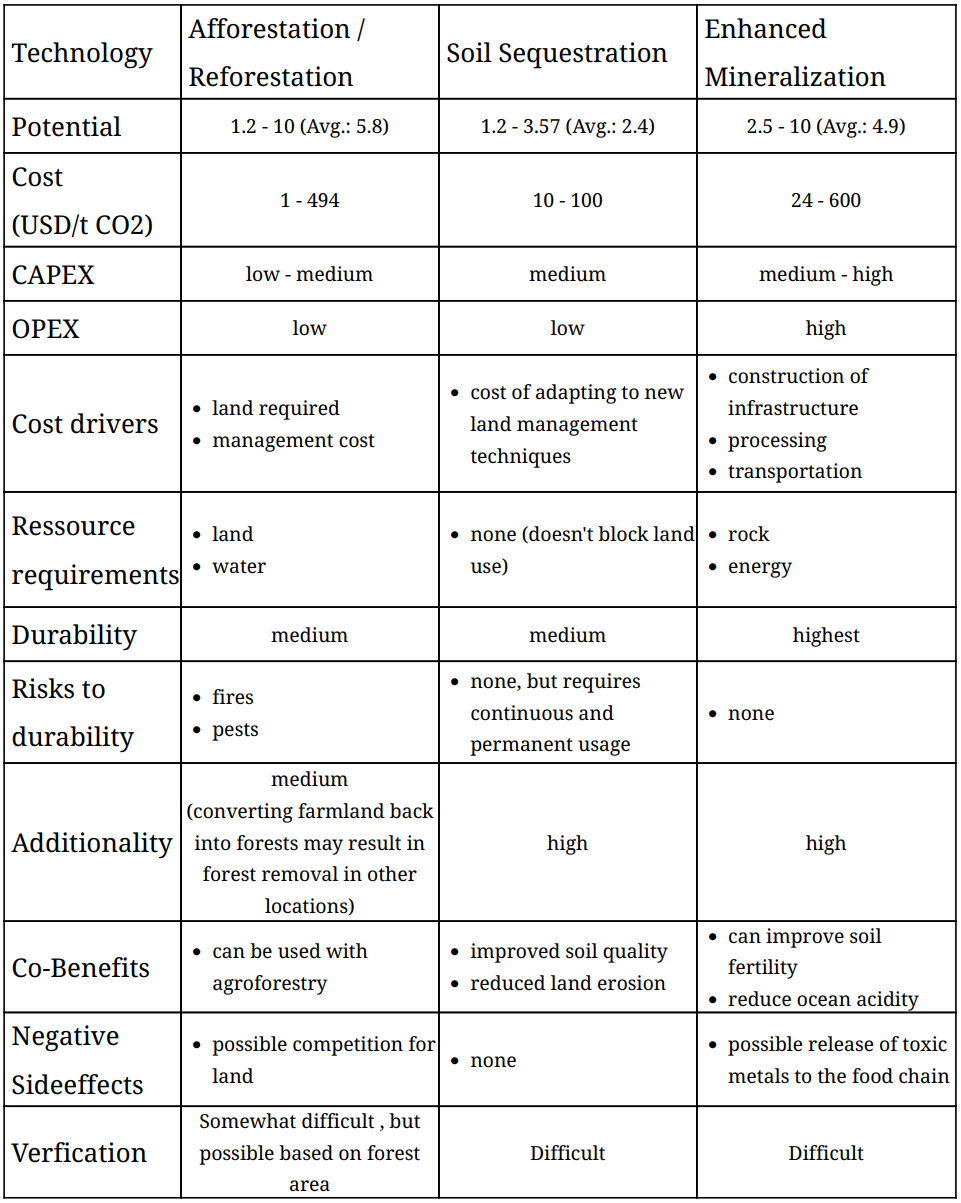
\includegraphics[width=\textwidth]{figures/table1.png}